% You should title the file with a .tex extension (hw1.tex, for example)
\documentclass[a4paper, 11pt]{article}

\usepackage{amsmath}
\usepackage{amssymb}
\usepackage{fancyhdr}
\usepackage{graphicx}

\usepackage[margin=1in]{geometry}
\usepackage{tikz}
\usetikzlibrary{automata,positioning,arrows}
\newcommand{\question}[2] {\vspace{.25in} \hrule\vspace{0.5em}
	\noindent{\bf #1: #2} \vspace{0.5em}
	\hrule \vspace{.10in}}
\renewcommand{\part}[1] {\vspace{.10in} {\bf (#1)}}

\newcommand{\myname}{Possawat Sanorkam}
\newcommand{\myemail}{possawat2017@hotmail.com}
\newcommand{\myhwnum}{2}

\setlength{\parindent}{0pt}
\setlength{\parskip}{5pt plus 1pt}

\pagestyle{fancyplain}
\lhead{\fancyplain{}{\textbf{HW\myhwnum}}}      % Note the different brackets!
\rhead{\fancyplain{}{\myname\\ \myemail}}
\chead{\fancyplain{}{ICCS310}}

\begin{document}
	
	\medskip                        % Skip a "medium" amount of space
	% (latex determines what medium is)
	% Also try: \bigskip, \littleskip
	
	\thispagestyle{plain}
	\begin{center}                  % Center the following lines
		{\Large ICCS310: Assignment \myhwnum} \\
		\myname \\
		\myemail \\
		\today \\
	\end{center}
	
	\question{1}{Regex to NFA/DFA} %don't delete yet:(}
	
	\part{1} $a(abb)^* + b $
	
	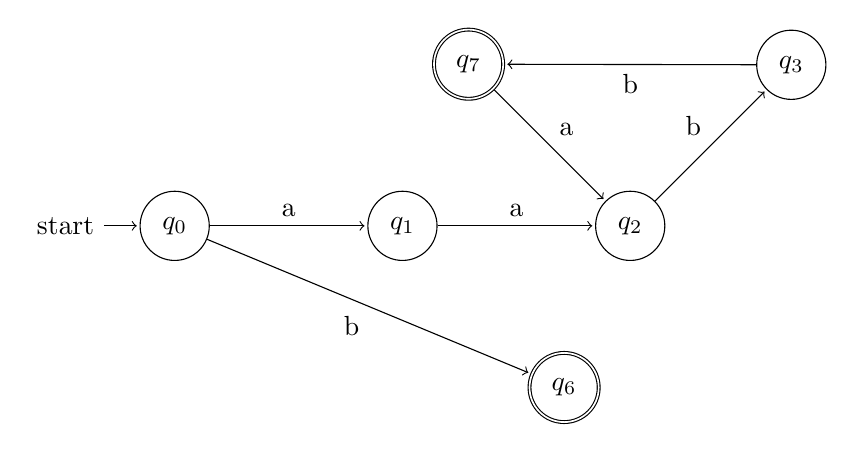
\begin{tikzpicture}[shorten >=1pt,node distance=2cm,auto] 
	\node[state,initial] (q_0)   {$q_0$}; 
	\node[state] (q_1) [ right=of q_0] {$q_1$}; 
	\node[state] (q_2) [ right=of q_1] {$q_2$}; 
	\node[state] (q_3) [above right=of q_2] {$q_3$}; 
	\node[state,accepting](q_6) [below right=of q_1] {$q_6$};	
	\node[state,accepting](q_7) [above left=of q_2] {$q_7$};
	\path[->] 
	(q_0) edge  node {a} (q_1)
	edge [swap] node {b} (q_6)
	(q_1) edge  node {a} (q_2)
	(q_2) edge  node {b} (q_3)
	(q_3) edge  node {b} (q_7)
	(q_7) edge  node {a} (q_2);

	\end{tikzpicture}
	
	\part{2} $(a + b)^* aa(a + b)^*$
	
	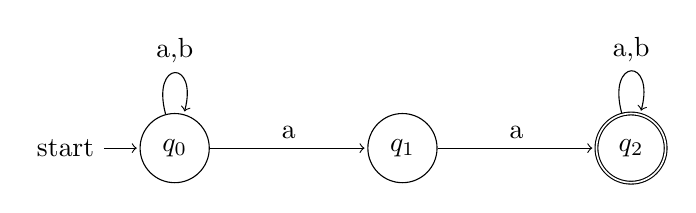
\begin{tikzpicture}[shorten >=1pt,node distance=2cm,auto] 
	\node[state,initial] (q_0)   {$q_0$}; 
	\node[state] (q_1) [right=of q_0] {$q_1$}; 
	\node[state,accepting](q_2) [right=of q_1] {$q_2$};
	\path[->] 
	(q_0) edge [loop above] node {a,b} ()
	edge  node {a} (q_1)
	(q_1) edge node {a} (q_2)
	(q_2) edge [loop above] node {a,b} ();
	\end{tikzpicture}

	\part{3} $a^+ + (ab)^+$
	
	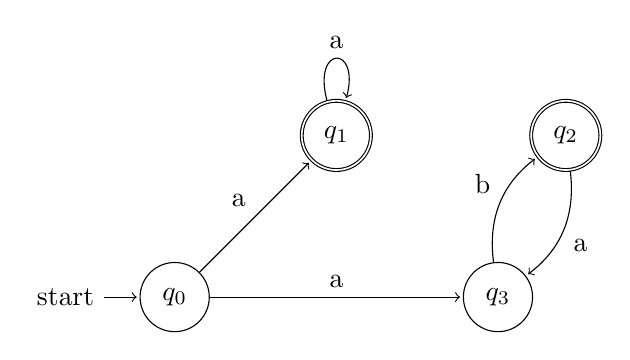
\begin{tikzpicture}[shorten >=1pt,node distance=2cm,auto] 
	\node[state,initial] (q_0)   {$q_0$}; 
	\node[state,accepting] (q_1) [above right=of q_0] {$q_1$}; 
	\node[state,accepting](q_2) [right=of q_1] {$q_2$};
	\node[state] (q_3) [below right=of q_1] {$q_3$}; 
	\path[->] 
	(q_0) edge  node {a} (q_1)
	edge node {a} (q_3)
	(q_1) edge [loop above] node {a} ()
	(q_2) edge [bend left]  node {a} (q_3)
	(q_3) edge [bend left]  node {b} (q_2);
	\end{tikzpicture}
	
	\question{2}{Finite-State Machines to Regex}
	
	\part{1} $ \varnothing^* $ (Rejecting any input)
	
	\part{2} $a^* + a^*b^+a^+b$ (Contains only $a$s or any pattern of $a$s to $b$s to $a$s to $b$s.)
	
	\question{3}{Binary Addition}
	
	Prove that in any set of $n +1$ numbers from $\{1, . . . , 2n\}$, there are always two numbers that are consecutive.
	
	{\em Proof}: Assume for the sake of contradiction that there is no two numbers that are consecutive given any set of $n +1$ numbers from $\{1, . . . , 2n\}$. Let $A$ be the set of $n +1$ numbers from $\{1, . . . , 2n\}$. Using pigeonhole principle, the required size of $A$ is too large to prevent consecutive numbers because the when the size of $A$ is n we could use the set of odd natural number or even natural number where all elements in $A$ is less than $n$. However, the last number to be added will contradict to our assumption that no two numbers are consecutive since there would be no other number to pick, except the consecutive number from $\{1, . . . , 2n\}$. Hence, $A$ is contradicting to our assumption.
	
	Therefore, any set of $n +1$ numbers from $\{1, . . . , 2n\}$, there are always two numbers that are consecutive.$\square$
	
	
	\question{4}{Division Operation?}
	
	Let $G = (V, E )$ be an undirected graph. Show that G contains two nodes that have equal degrees.
	
	{\em Proof}: Without loss of generality, assume for the sake of contradiction that $G$ is an undirected graph with no loops which has $n$ vertices and every vertices have different degrees. Let D be the set of degrees for each vertex, $D = \{d_1, d_2, d_3, \dots , d_n\}$. Then, $D = \{0,2,...,n-1\}$, since the number of degree is between $0$ to $n-1$.  From observation, we have that there is a vertex with degree $n-1$ and a vertex with degree $0$ which is not possible for any undirected graph. Hence, $D$ contradicted to what we assumed.
	
	Therefore, if $G = (V, E )$ is an undirected graph, then $G$ contains two nodes that have equal degrees.$\square$
	
	\question{5}{Does It Accept Everything?}
	Let $\sum = \{a, b, c\}$.
	
	\part{1} The language of strings on $\sum$ whose length is divisible by 5.
	
	{\em Solution}:
	\begin{figure}[htbp]
		\centering
		\includegraphics[width=\linewidth]{figures/1.jpg}
	\end{figure}
	
	Let n be the length of the input string.
	
	$S_0$ represents the state where $0 \pmod{5} \equiv n$.\\
	$S_1$ represents the state where $1 \pmod{5} \equiv n$.\\
	$S_2$ represents the state where $2 \pmod{5} \equiv n$.\\
	$S_3$ represents the state where $3 \pmod{5} \equiv n$.\\
	$S_4$ represents the state where $4 \pmod{5} \equiv n$.
	
	So, the accepting state is $S_0$ since this state means the length is divisible by 5.
		
	\part{2} The language of strings on $\sum$ whose length is either even or divisible by 5 (or both).
	
	{\em Solution}:
	
	\begin{figure}[htbp]
		\centering
		\includegraphics[width=\linewidth]{figures/2.jpg}
	\end{figure}
	Let $n$ be the length of the input string.
	
	$S_0$ represents the state where $0 \pmod{5} \equiv n$.\\
	$S_1$ represents the state where $1 \pmod{5} \equiv n$.\\
	$S_2$ represents the state where $2 \pmod{5} \equiv n$.\\
	$S_3$ represents the state where $3 \pmod{5} \equiv n$.\\
	$S_4$ represents the state where $4 \pmod{5} \equiv n$.
	
	So, the accepting state is $S_0, S_2, S_4$ since this state means the length is either even or divisible by 5
	
	\part{3} The language of strings on $\sum$ that has at least one a and contains an even number of $b$s.
	
	{\em Solution}:
	\begin{figure}[htbp]
		\centering
		\includegraphics[width=\linewidth]{figures/3.jpg}
	\end{figure}

	Let $K$ be any input string from language set $\sum$.
	
	$S_\epsilon$ represents the state where there is not a match with the pattern.\\
	$S_a$ represents the state where K has at least one $a$ and contains an even number of $b$s.\\
	$S_{ba}$ represents the state where K has at least one $a$ and contains an odd number of $b$s.\\
	$S_b$ represents the state where K has no $a$ and contains an odd number of $b$s.
	
	So, the accepting state is $S_a$ since this state means the input string has at least one $a$ and contains an even number of $b$s.
	\\\\\\\\\\\\\\\\\\\\\\\\\\
	
	
	\question{6}{All The Same?}
	\part{1} Let $L_2 = \{x \in \sum^{*}: \text{the 2nd-to-last symbol of x is 1}\}$. Draw a DFA with 4 states that accepts $L_2$.
	
	{\em Solution}:
	\begin{figure}[htbp]
		\centering
		\includegraphics[width=\linewidth]{figures/4.jpg}
	\end{figure}
	
	$S_\epsilon$ represents the state where there is not a match with the pattern.\\
	$S_{n-1}$ represents the state where $1$ is found but at the last position.\\
	$S_{1}$ represents the state where $1$ is found at the second-to-last position, and the last alphabet is $1$.\\
	$S_0$ represents the state where $1$ is found at the second-to-last position, and the last alphabet is $0$.\\
	
	So, the accepting state is $S_1 \text{ and } S_0$ since these states mean the second-to-last symbol of input string is $1$.
	
	
	\part{2} Show that any DFA that correctly recognizes $L_2$ must have at least 4 states.
	
	{\em Proof}: Without loss of generality, let us assume for the sake of contradiction that there exist D, a DFA that correctly recognizes $L_2$ using less than 4 states. Let D be a DFA that has 3 states. By the Pigeonhole Principle, if we choose 4 strings over $\sum$, then at least two of those strings must end at the same state $q$. Let $t_i$ and $t_j$ be these 2 strings that satisfies the above. Let $t_0 = \epsilon, t_1 = 1, t_2 = 11, t_3 = 111$. For one of the pairs of strings, the supposed 3-state DFA is forced into the same state for both strings, and $t_{ix} \text{ and } t_{jx}$ must be both accepted or both rejected, for
	any string x. We want to show, for each possible pair, that this is not true. 
	
	First pair, $t_0 \text{ and } t_1$, and choose $x = 1010$. $t_0x = 1010, t_{1x} = 11010$, both rejected.
	
	Second pair, $t_0 \text{ and } t_2$, and choose $x = 00$. $t_0x = 00, t_{1x} = 100$, both rejected.
	
	Third pair, $t_0 \text{ and } t_3$, and choose $x = 00$. $t_0x = 00, t_{1x} = 100$, both rejected.
	
	First pair, $t_1 \text{ and } t_2$, and choose $x = 00$. $t_0x = 00, t_{1x} = 100$, both rejected.
	
	First pair, $t_1 \text{ and } t_3$, and choose $x = 00$. $t_0x = 00, t_{1x} = 100$, both rejected.
	
	First pair, $t_2 \text{ and } t_3$, and choose $x = 00$. $t_0x = 00, t_{1x} = 100$, both rejected.
	
	%So, to check whether a string can be recognize requires 4 steps. 
	%The first step is to check whether we found 1 yet, because it could the the second last position symbol we need. 
	%The second step is to check whether the next state is 1 or zero, and there will be two cases to consider, the first case is that the second-to-last symbol of $x$ is 1 and the next symbol is 1 and another case is the second-to-last symbol of $x$ is 1 and the next symbol is 0. We have to change state every time any 0 showed up after we found the first 1. So, we need at least 4 steps to correctly recognize $L_2$. Using pigeonhole principle, the least number of states required is 4 since we showed that 4 different states are needed but the number of states in D is smaller than 4 and there are some patterns of symbols such as 1010 and 1101 that could end up in the same state. Hence, D cannot correctly recognize $L_2$ with only 3 states which is contradicting to what our assumption.
	
	Therefore, any DFA that correctly recognizes $L_2$ must have at least 4 states. $\square$
	\\\\\\\\\\
	\question{7}{Digit Sum}
	\part{1} $L = \{x \in \sum^{*}: \texttt{DIGITSUM(x)} \text{is divisible by 3}\}$. Draw a DFA that recognizes $L$. Explain what each of your states represents.
	
	{\em Solution}:
	\begin{figure}[htbp]
		\centering
		\includegraphics[width=400px]{figures/5.jpg}
	\end{figure}
	
	Let $n_i$ be the accumulating sum of input string at position $i$.
	
	$S_0$ represents the state where $0 \pmod{3} \equiv n_i$.\\
	$S_1$ represents the state where $1 \pmod{3} \equiv n_i$.\\
	$S_2$ represents the state where $2 \pmod{3} \equiv n_i$.\\
	
	So, the accepting state is $S_0$ since this state means $\texttt{DIGITSUM(x)} \text{is divisible by 3}$ where $x \in \sum^{*}$.
\end{document}